\newpage
\section{The RS02 codec}

This section describes the dvdisaster RS02 Reed-Solomon codec.
It was developed during the winter of 2005/2006 in order to facilitate
augmenting iso images directly with error correction data.

RS02 is based on the Reed-Solomon encoders and decoders 
introduced with RS01, but focuses exclusively on augmenting
iso images. The allocation of data sectors within an ecc block 
follows a similar scheme as in RS01. However the layout of the
parity bytes is vastly different between RS01 and RS02, as the codec must
cope with any parity sector being damaged or unreadable. 
Consequently a RS02 image can lose as many sectors as 
allowed by the redundancy of
the error correction data, and the lost sectors can be any
combination of data and parity sectors, as it is expected from
a Reed-Solomon scheme.

\smallskip

Unlike RS01, which will be completely superseded by RS03 soon,
the case of RS02 vs. RS03 still remains open, as both codecs
have their individual strengths. RS02 is slightly more space
efficient than RS03, so on CD media RS02 might provide
slightly more redundancy (typically one additional root) than RS03. 
This effect will be less
pronounced on larger media like DVD and BD. 
RS02 images can be augmented to an arbitrary size which may
be smaller than the maximum medium size, while RS03 requires
augmenting the image to the full medium size.
This might favour RS02 for working on images which are only
30\% or less of the medium size, as they can be encoded with
less than the maximum of 170 roots 
(the maximum redundancy requires lots of time to compute, producing
a three-fold redundancy which may not be needed in all cases). 
On the other hand RS03 will counter
the performance argument since it can encode at least 
20 times faster than RS02 on multi-core architectures, 
because RS02 encoding can not be parallelized. 
See the end of section \ref{rs01}  for a speed comparison of RS01 vs. RS03; 
RS01 and RS02 are very similar performance-wise.
Finally, the data layout of RS03 does not depend on interspersed
ecc headers which gives it a better robustness over RS02;
see subsection \ref{layout-logical-two} for details.

\subsection{Physical layout}

\begin{figure}
 \begin{center}
 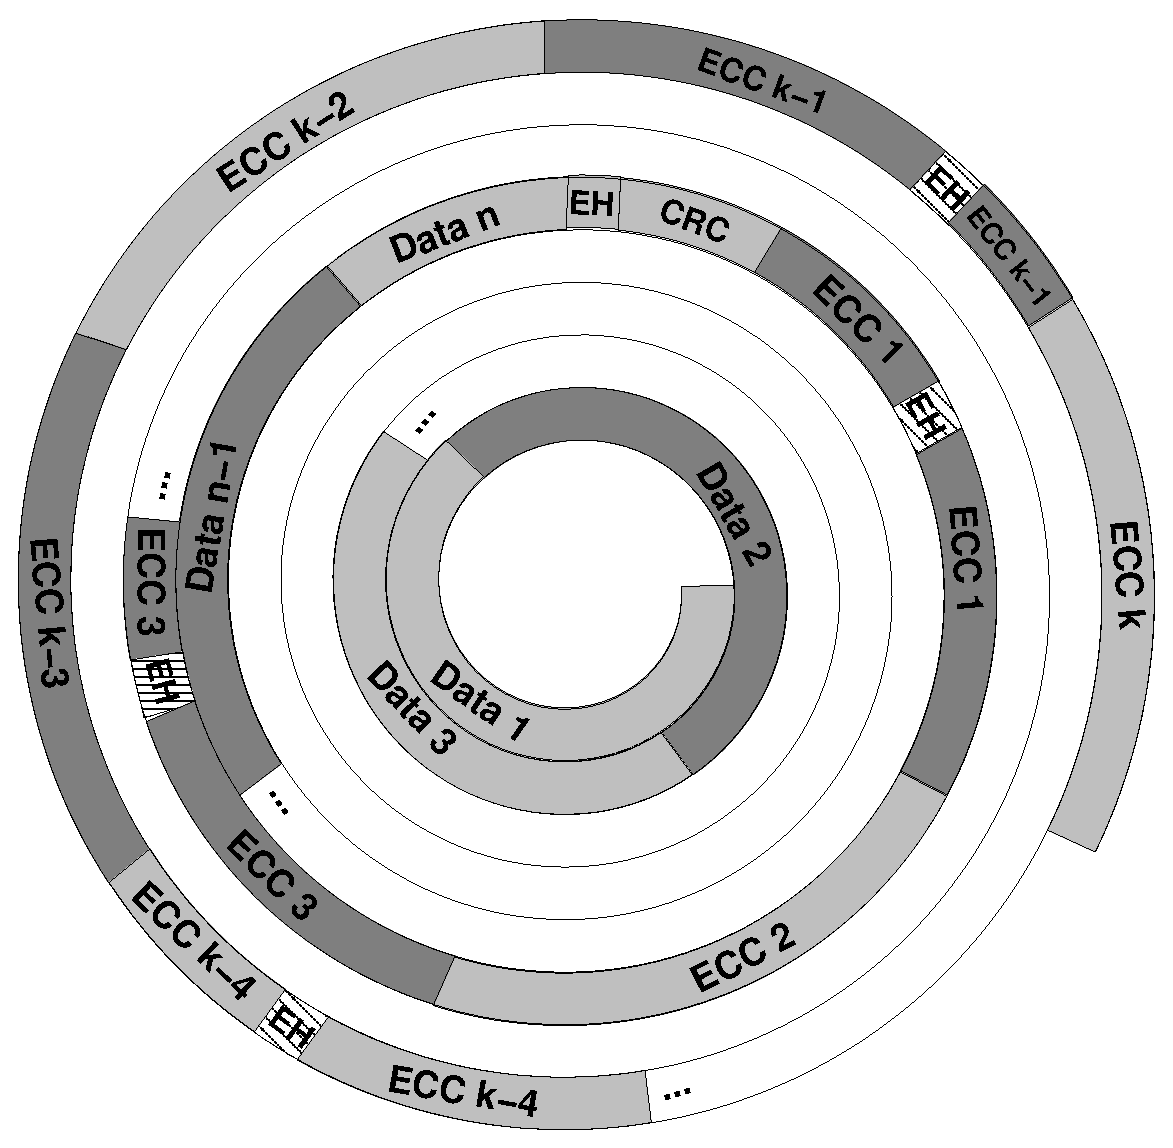
\includegraphics[width=10cm]{spiral-rs02.eps}
 \caption{Physical RS02 layout}
 \label{layout-phy-two}
 \end{center}
\end{figure}

RS02 must be applied to the .iso image before it is written to
the medium. Additional sectors are appended to the .iso image 
containing the parity data. The data structures of the .iso image
are not changed to reflect the new image size, so the original
part of the augmented .iso image remains untouched. The parity
sectors can be removed from the augmented image by simply 
truncating the .iso image to its original sector size; the resulting
image file will have the same contents as prior to the augmentation.
As a side effect, the parity data is invisible to applications reading
the medium at the filesystem level, including most hardware media
players. If you find a player which gets confused by media containing
RS02 (or RS03) parity, please consider telling the dvdisaster project about it. As of this writing,
not a single device has been reported to run into problems with
the RS02 data scheme. The RS02 augmented image might conflict with
optical media writing software, though. If the writing software
decides the image length by looking at the iso filesystem structures,
the parity data portion of the image might not be written to the medium.
Most current writing programs do however measure the .iso image by examining
its file size, and will transfer the parity data correctly. To be sure you
should follow the steps described under ``Testing image compatibility''
at the dvdisaster site (\url{http://dvdisaster.net/en/howtos92.html}) once
before using each version of your optical media authoring software.

Like the other dvdisaster codecs, RS02 is based on a  RS(255,k) Reed-Solomon code
with each ecc block being comprised of $n$ data bytes and $k$ parity bytes, and
$n+k=255$. The $n$ data bytes comprise the .iso image which will be
written to the medium, and the additional ecc header and CRC checksums added
by dvdisaster. Reed-Solomon encoding works best when errors are
distributed evenly over all ecc blocks. Therefore we must strive to distribute
the ecc blocks evenly over the medium surface. To facilitate such mapping,
dvdisaster logically divides the medium into 255 logical units which are called
``layers'' for historical reasons. 
Figure \ref{layout-phy-two} shows how the medium is divided into $n$ data layers
and $k$ ecc layers, with $n + k = 255$. Ecc blocks are
created by taking on byte from each layer as shown in fig. \ref{layout-logical-two}
on the following page. This distributes the ecc block reasonably good over
the medium surface. 
All layers have the same length in bytes, with the possible exception of
data layer $n$. As the .iso image size plus the size of one ecc header and the CRC data
is usually not a multiple of the layer size, the $n$-th data layer may be shorter
than the layer size and considered to be filled up with a virtual zero padding. 
The zero padding is not written out to the augmented image (note that data layer $n$
is intentionally drawn shorter in fig. \ref{layout-phy-two}), but it is used in the
calculation of the respective parity bytes.

\newpage

\subsection{Logical layout}
\label{sec-layout-logical-two}

\begin{figure}
 \begin{center}
 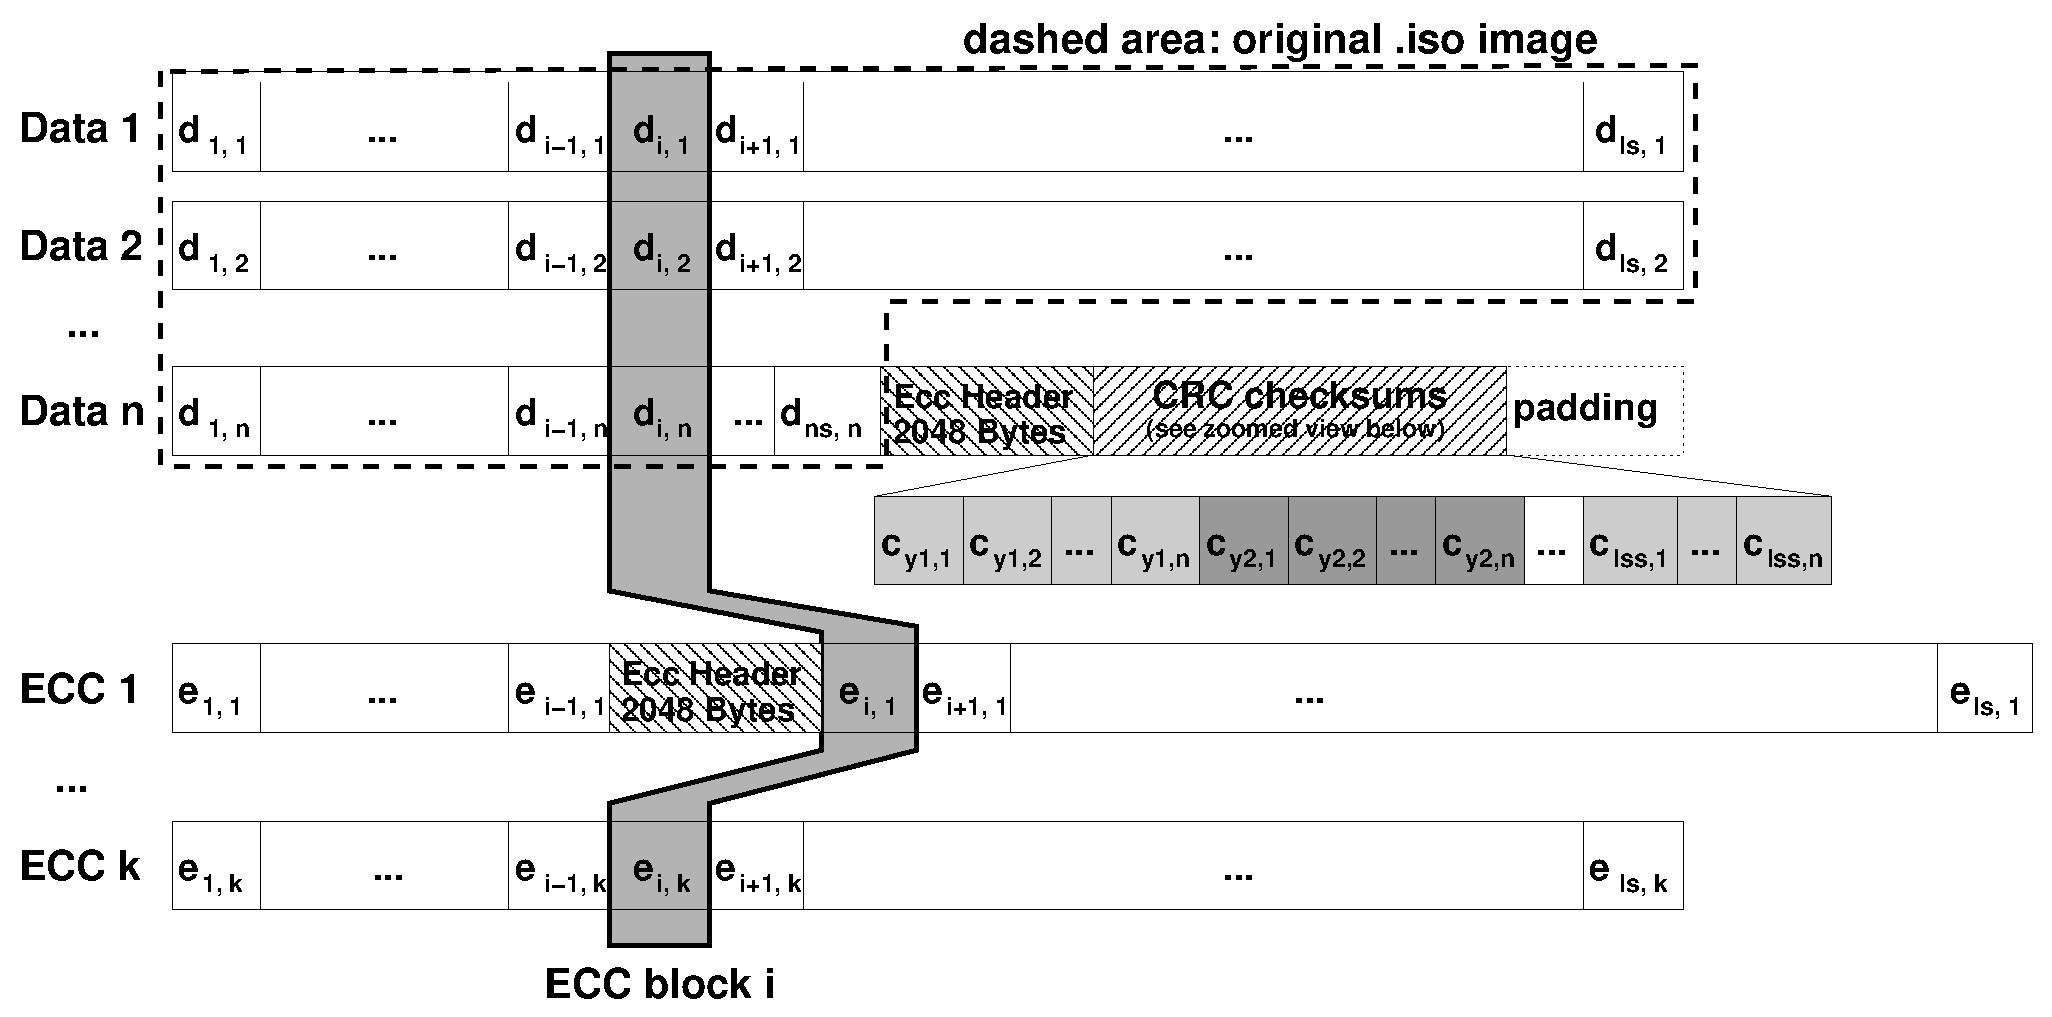
\includegraphics[width=\textwidth]{rs02-layout.eps}
 \caption{Logical RS02 layout}
 \label{layout-logical-two}
 \end{center}
\end{figure}

The data layout in the augmented image is shown in figure \ref{layout-logical-two}.
Note that in this figure the data is byte-indexed; e.g. $d_{1,1}$ denotes the
first data byte in the augmented image. Each layer has a length of
$ls$ bytes, with the exception of data layer $n$ which may be shortened (see subsection \ref{calc-two} for an exact calculation of its size). 
Some ecc layers my be interleaved with redundant copies of the ecc header. 
The ecc header size is not included in the respective ecc layer size.

\paragraph{Data layers.} A data layer index $d_{i,j}$ refers to the $i$-th byte in the $j$-th data layer.
The $n$ data layers are mapped in a linear fashion to the original iso image.
$d_{1,1}$ maps to the first .iso image byte, and $d_{ns,n}$ maps to the last .iso image
byte ($ns$ is the number of remaining iso image bytes in the $n$-th data layer). 

The last data layer is special because it does not only contain the rest of the iso image,
but also the ecc header and the CRC checksums. These extensions 
are logically treated as a part of the iso image; their contents are used in the
ecc data calculation and are therefore protected by the ecc data.
The ecc header follows immediately after byte $d_{ns,n}$ and is 4096 bytes long.
Its format is described in appendix \ref{eh}. For RS02, only the data fields
marked with ``all'' or ``RS02'' are relevant; all other fields should be set to zero.

Data layer $n$ does also contain the CRC32 checksums of each data sector
upto the ecc header. If the .iso image contains $s$ sectors, 
then the CRC field contains $4s$ bytes, rounded up
to the nearest multiple of 2048. 
CRC32 checksums are calculated over a whole CD sector comprising 2048 bytes.
Let $c_{y,j}$ be the 4-byte checksum of the $y$-th sector in the $j$-th layer
and $lss$ be the number of sectors in each layer.
Then $c_{y,j}$ = CRC32($d_{2048*y,j}$, $d_{2048*y+1,j}$, \dots, $d_{2048*y+2047,j}$).  
 
$y_1$ is usually not the first sector in the layer, but a later sector.
In general, $y_i$ = $(i+offset)$ mod $lss$. The offset is introduced to restore
the CRC32 sums of ecc block $i+1$ during the correction of ecc block $i$.
This helps if the data portion of the image is corrupted with wrong byte values and
the sectors containing the CRC32 sums have been lost. 
The error correction will start at the ecc block $i$ which is determined
by the offset, and whose CRC32 checksums are stored in the ecc header (at least one
ecc header will be recovered before any error correction can begin). Correcting
ecc block $i$ will recover the CRC32 checksums for ecc block $i+1$ in the image
(and possibly some more in advance, as less than 2048 bytes are required for
one set of checksums). This makes it possible to detect corrupted bytes by the
checksums and flag them as erasures which effectively doubles the error correction
capabilities of the Reed-Solomon code.

\paragraph{Ecc layers.} For an image augmented with $k$ roots, the parity bytes
will be spread over $k$ ecc layers. In order to calculate the first ecc block,
bytes $d_{1,1}$ to $d_{1,n}$ are taken from the $n$ data layers. The RS(255,k) code
is calculated (see appendix \ref{rs} for its parameters) and the resulting $k$
parity bytes $e_{1,1}$ to $e_{1,k}$ are stored in the $k$ ecc layers. 
The next ecc blocks are calculated and stored accordingly; ecc block $i$ 
is marked grey in the figure.
Care must be taken to honour the non-linear mapping of
ecc layer bytes as the ecc area is interleaved with 20-40 copies of the ecc header.
The ecc header copies are placed at sector addresses whose numbers 
are large powers of two. This makes it possible to heuristically search for them
during the decoding boot-strap process 
when no other information (image size, layer size, etc.) is yet available.
See section \ref{search-two} on the search heuristics and section \ref{addressing-two}
on calculating ecc bytes positions from the non-linear mapping. 

\subsection{Calculating the image layout for encoding}

The image layout can be either computed automatically to fill up
the medium as much as possible, or by user selected criteria such
as a maximum image size or a specified redundancy.

\subsubsection{Automatic layout calculation}
\label{calc-two}

The only available inputs to automatic layout detection are
the .iso image size and a table of maximum media sizes (see
tab. \ref{layout-size-table} in the RS03 section for the
respective values). From the media size table the smallest
possible medium  is chosen which can contain the .iso image.
In some border cases, with e.g. the .iso image being only
100 sectors smaller than the medium capacity, the automatic
layout calculation will fail later due to insufficient space
on the medium. In such cases, the user must decide between
choosing the next larger medium size or splitting the image
contents onto two media by himself (splitting a 700MiB CD image 
onto two CDs may be better than writing it to a DVD).

\smallskip

From now on, all calculations are given in numbers of 2048K 
sectors or sectors addresses
unless noted otherwise. The number of sectors required for the
CRC checksums can be directly computed from the .iso image size:

\[
crc\; sectors = \left\lceil\frac{4 * iso\; image\; sectors}{2048}\right\rceil
\]

The total accumulated size of all data layers is the sum of the
.iso image size, the number of crc sectors and the two sectors required
for the ecc header. Since these sectors are protected by the parity,
they are called {\em protected sectors}:

\[protected\; sectors = iso\; image\; size + 2 + crc\; sectors\]
 
These calculations also produce two important sector addresses within
the augmented image:

\begin{itemize}
\item The sector with address {\em iso image size} marks the location
of the ecc header; and
\item The sector at address $iso\; image\; size + 2$ marks the beginning
of the CRC checksum data.
\end{itemize}

The next step is to partition the {\em protected sectors} and the remaining
medium space into an optimal layer size. It is carried out iteratively.

\smallskip

For an approximate start, we determine the free space on the medium:

\[free\; space = medium\; capacity - protected\; sectors\]

and estimate a preliminary value for the number of roots and data layers:

\[k\; roots = min\left(170, \quad\left\lfloor\frac{255 * free\; space}{medium\; capacity}\right\rfloor\right)\]

\[n\; data = 255 - k\; roots\]

The maximum number of roots is capped at 170 which is approximately a three-fold
redundancy. Larger values would get too computationally expensive.

\smallskip

The preliminary layer size is then:

\[preliminary\; layer\; size = \left\lceil\frac{protected\; sectors}{n\; data}\right\rceil\]

and the expected size of the parity layers is:

\[preliminary\; ecc\; size = k\; roots * preliminary\; layer\; size\]

\smallskip

% TODO: implement in codec
\begin{comment}

From these values we iteratively compute a $2^p$ which has about 20-40 multiples
in the {\em preliminary ecc size} address space. This value will be used
for interleaving the ecc header copies with the ecc layers:

\smallskip

{\tt
p := 5

while($\frac{preliminary\;ecc\;size}{2^p} > 40$)

\quad p := p + 1}  
\end{comment}

From these values we compute a $2^p$ which has about 20-40 multiples
in the {\em preliminary ecc size} address space. This value will be used
for interleaving the ecc header copies with the ecc layers:

\[ p = \left\lceil log_2\; \frac{preliminary\;ecc\;size}{40} \right\rceil \]

%\[ p = \left\lceil \frac{log\; \frac{preliminary\;ecc\;size}{40}}{log\; 2} \right\rceil \]


\smallskip

Now the chosen values might be actually too big since we haven't taken
the ecc header copies into account. 
So the final task is to add up the number pf parity sectors and ecc header
copies. If these fit into the free medium space, we are done; otherwise
the calculations are done again with one root less.

\newpage

\bigskip

while($n\; roots > 7$)

\smallskip

\quad $layer\; size := \left\lceil\frac{protected\; sectors}{n\; data}\right\rceil$

\smallskip

\quad $ecc\; size := n\; roots * layer\; size$

\smallskip

\quad $first\; ecc\; header\; repeat\; addr := \left\lceil\frac{protected\; sectors}{2^p}\right\rceil * 2^p$ 

\smallskip

\quad $space\; for\; interleaved\; sectors := protected\; sectors + ecc\; size - first\; ecc\; header\; repeat\; addr$

\smallskip

\quad $number\; of\; ecc\; copies := \left\lfloor\frac{space\; for\; interleaved\; sectors}{2^p - 2}\right\rfloor + 1$

\smallskip

\quad $total\; added\; sectors := 2 + crc\; sectors + ecc\; size + 2 * number\; of\; ecc\; copies$

\medskip

\quad If $iso\; image\; sectors + total\; added\; sectors < medium\; size$,
we have a valid layout: STOP.

\smallskip

\quad Otherwise, set $n\; roots := n\; roots - 1$ and $n\; data := 255 - n\; roots$
and do another iteration. 

\medskip

The iteration will either terminate with a valid layout or fail when
$n\; roots$ drops below the minimum redundancy of 8 roots. 

\subsubsection{Layout calculation by user selected criteria}

The user has several means of specifying a certain redundancy:

\paragraph{Specifying the maximum number of sectors for the augmented image.}

This case is simply handled by setting {\em medium capacity} to the user
selected sector size rather than using the maximum medium size from the
built-in table. Afterwards, calculations continue as described in
section \ref{calc-two}.

\paragraph{Specifying the number of roots to use.}

In this case we can skip the calculations for {\em free space} and
{\em k roots} as described in section \ref{calc-two}, and instead
set {\em k roots} directly to the user selected value. Then the
layout calculation proceeds as usual. 

\paragraph{Specifying the percentage of redundancy to use.}

For a given number of {\em k roots}, the resulting redundancy in percent is:

\[\frac{k\; roots \cdot 100}{255 - k\; roots}\]

Pick a suitable value for {\em k roots} so that the user selected value
is met or slightly exceeded. Proceed with the given number of roots
as described in the previous paragraph.

\subsubsection{Layout calculation from ecc header information}
\label{recalc-layout-header-two}

In a given ecc header struct {\em eh}, the number of sectors in the .iso
image is recorded as \mbox{\em eh-$>$sectors} 
and the number of roots is contained in \mbox{\em eh-$>$eccBytes}.
Calculation of the layout is done as shown in section \ref{calc-two}, 
with the exception of omitting the calculation for {\em free space} and
setting {\em k roots} directly to  \mbox{\em eh-$>$eccBytes}.

\subsection{Automatic layout calculation example}
\label{example-two}

Let's assume we are going to encode an .iso image of 295.000 sectors.
This is well below the CD medium capacity of 359.424 sectors, so we
start with:

\smallskip

$medium\; capacity = 359.424\; sectors$

$iso\; image\; size = 295.000\; sectors$

\medskip

The number of CRC sectors will be:

\smallskip

$crc\; sectors = \left\lfloor\frac{4 * 295.000}{2.048}\right\rfloor = 577\; sectors$

\medskip

The total size of all data layers is:

$protected\; sectors = 295.000 + 2 + 577 = 295.579\; sectors$

\bigskip

The next step is creating some preliminary starting values:

\smallskip

$free\; space = 359.424 - 295.579 = 63.845\; sectors$

\smallskip

$k\; roots = min\left(170, \left\lfloor\frac{255* 63.845}{359.424}\right\rfloor\right) = min(170, 45) = 45\; roots\; (or\; layers)$

\smallskip

$n\; data = 255 - 45 = 210\; layers$

\bigskip

Now some more preliminary values can be computed:

\smallskip

$preliminary\; layer\; size = \left\lceil\frac{295.579}{210}\right\rceil = 1.408\; sectors$

\smallskip

$preliminary\; ecc\; size = 45 * 1.408 = 63.360\; sectors$

\bigskip

Finally, we compute $p = 11$ since $\frac{63360}{2^{11}} = 30,9$.

\bigskip

Now the chosen values must be verified to produce a layout which is
still smaller than the image size. We compute (the first two values are already known):

\medskip

$layer\; size = \left\lceil\frac{295.579}{210}\right\rceil = 1.408\; sectors$

\smallskip

$ecc\; size = 45 * 1.408 = 63.360\; sectors$

\smallskip

$first\; ecc\; header\; repeat\; addr = \left\lceil\frac{295.579}{2048}\right\rceil * 2048 = 296.960$

\smallskip 

$space\; for\; interleaved\; sectors = 295.579 + 63.360 - 296.960 = 61.979\; sectors$

\smallskip

$number\; of\; ecc\; copies = \left\lfloor\frac{61.979}{2048-2}\right\rfloor + 1 = 31\; header\; repeats$

\smallskip

$total\; added\; sectors = 2 + 577 + 63.360 + 2 * 31 = 64.001\; sectors$

\medskip

This layout will generate an augmented image containing
$295.000 + 64.001 = 359.001$ sectors which is 
less than the medium capacity of 359.424 sectors
and therefore accepted.

\subsection{Re-calculating the layout from defective media}
\label{search-two}

In order to recover a defective medium, at least one ecc header must
remain readable and be located by the following heuristic. This
is a major difference to RS03, which has more and different means
for bootstrapping the recovery (see section \ref{recover} for details).
Once one ecc header has been recovered, the ecc data layout can be
calculated as described in section \ref{recalc-layout-header-two}.
From this point, the error correction is done using the parameters
and data described in section \ref{encoding-two}.

\smallskip

If the medium is not damaged or only slightly damaged, the following
short cut might work: The size of the .iso image can be determined
from the iso file system header. Then the ecc header immediately
following the .iso image part of the augmented image is either
located at sector number $iso\;image\;size$ or $iso\;image\;size + 150$.
The latter case arises because some popular CD authoring software
appends 150 padding sectors to any .iso image it creates. 

\smallskip

If the short cut does not work due to the required sectors being damaged,
the following strategy is employed. The size of the augmented image
can always be determined; it can either be queried from the drive or
it is the file size of a file-based image. Then apply the following
algorithm:

\bigskip

$p = \left\lfloor log_2(image\; size)\right\rfloor$

while $p > 32$

\quad $pos = \left\lfloor\frac{image\; size}{2^p}\right\rfloor \cdot 2^p$

\smallskip

\quad while $pos > 0$

\qquad if {\em sector at pos} is a valid ecc header: STOP.

\qquad if {\em sector at pos} is unreadable, set $pos := pos - 2^p$ .

\hspace*{13mm} Continue with inner while loop.

\qquad if {\em sector at pos} is readable and not a ecc header, set $p := p -1$ .

\hspace*{13mm} Continue with outer while loop.

\bigskip

In order to test for a valid ecc header, check that {\em ec-$>$cookie}
equals the 16-byte string ``*dvdisaster*RS02''. Then check that the
CRC32 sum of the ecc header matches the value recorded in {\em eh-$>$selfCRC},
with {\em eh-$>$selfCRC} set to the byte sequence 0x47,0x50,0x4c,0x00
for the purpose of calculating the CRC32 sum.

\medskip

Please notice that during testing of the sectors at multiples of $2^{(p-1)}$,
all sectors previously tested for $2^p$ will be examined again. It is therefore
highly recommended to cache results from previous iterations of the outer
while loop, especially when reading sectors from the optical medium.



\subsection{Sector addressing and initialization scheme}
\label{addressing-two}

For encoding and decoding purposes it is required to retrieve the
{\em i-th} sector from the {\em j-th} data or ecc layers, e.g. to calculate
the corresponding sector number in the augmented image. 
The reverse calculation is also needed, e.g. to calculate the
corresponding layer and sector index for a given sector number
in the augmented image.

\smallskip

Bear in mind that as shown in figure \ref{layout-logical-two}, an augmented image 
is divided into two logical parts. There is a data area containing 
the .iso image contents, the first ecc header and the CRC checksums.
The data area is protected by the parity in the ecc area, which contains
the parity data interleaved with copies of the ecc header. 

\smallskip

In order to carry out the calculations described below, the following
values from the layout calculation (see section \ref{calc-two} are required:

\bigskip

\begin{tabular}{lp{10cm}}
{\em protected sectors} & the size of the data part in sectors \\
{\em layer size} & the number of sectors per layer \\
{\em $2^p$} & the modulo value for locating ecc header copies \\
\end{tabular}

\paragraph{Converting (layer, sector index) pairs into image sector numbers.}

The {\em i-th} sector of data layer {\em j} has the following address $s$ in the image:

\[s = j \cdot layer\; size + i\]

If $s >= protected\; sectors$, $s$ is a padding sector which must not be read 
from the image file, but created in memory (see the paragraph on initialization below).

\bigskip

To calculate the sector address $es$ of the {\em i-th} sector from the {\em j-th} 
ecc layer, the non-linear mapping of the ecc sectors has to be taken into account.
The index of the first interleaved ecc header is:

\[ first\; interleaved = \left\lceil\frac{protected\; sectors}{2^p}\right\rceil \cdot 2^p\]

Since {\em protected sectors} is equal to the address of the first ecc sector in the image,
the amount of ecc sectors before the first interleaved ecc header is:

\[ base\; ecc\; sectors = first\; interleaved - protected\; sectors\]

The ecc sector we are looking for would have the following index if ecc
sectors were linearly mapped:

\[ ecc\; index = j \cdot layer\; size + i\]

If {\em ecc index $<$ base ecc sectors}, $es$ = {\em protected sectors} + {\em ecc index}.
Otherwise, the non-linear mapping must be taken into account. The number of interleaved
ecc headers before the (currently unknown) sector position $es$ is:

\[ interleaved\; headers = \left\lfloor\frac{ecc\; index - base\; ecc\; sectors}{2^p - 2}\right\rfloor \]

Therfore the position of the ecc sector in the augmented image is:

\[ es = protected\; sectors + ecc\; index + 2 \cdot interleaved\; headers + 2 \] 

\paragraph{Example.} To continue the example from section \ref{example-two}, the
position of the 17th ecc sector in the 3rd ecc layer shall be computed. The relevant
layout values are:

\smallskip

\begin{center}
\begin{tabular}{rll}
{\em protected sectors} & = & 295.579 \\
{\em layer size} & = & 1.408 \\
{\em $2^p$} & = & 2.048 \\
\end{tabular}
\end{center}

The first interleaved ecc header is at position:

\[ first\; interleaved = \left\lceil\frac{295.579}{2.048}\right\rceil \cdot 2.048 = 296.960 \]

Before the first interleaved ecc header,

\[ base\; ecc\; sectors = 296.960 - 295.579 = 1.381 \]

ecc sectors have been stored. The linear index of the sought ecc sector is:

\[ ecc\; index = 3 \cdot 1.408 + 17 = 4.241 \]

Since 4.241 $\ge$ 1.381, the embedded ecc headers must be taken into account. There are

\[ interleaved \; headers = \left\lfloor\frac{4.241 - 1.381}{2.048-2}\right\rfloor = 1 \]

interleaved ecc headers, each containing 2 physical sectors. Therefore the position
of the sought ecc sector in the image is:

\[ es = 295.579 + 4.241 + 2 + 2 = 299.824 \]

\bigskip

{\bf Converting image sector numbers into (layer, sector index pairs).}

\smallskip

If the sector number $s$ $<$ {\em protected sectors}, the sector will map to the data part
as follows:

\[layer = \left\lfloor s\; /\; layer\;size \right\rfloor\]
\[i = s \bmod layer\;size\]

Otherwise, the mapping to the ecc part is calculated as follows. The index of the first interleaved ecc header is:

\[ first\; interleaved = \left\lceil\frac{protected\; sectors}{2^p}\right\rceil \cdot 2^p\]

If $s\; mod\; 2^p \le 1$, the sector maps to the {\em n-th} interleaved ecc header, with:

\[n = \left\lfloor\frac{s - first\; interleaved}{2^p}\right\rfloor\] 

If $s < first\; interleaved$, the sector is an ecc parity sector with the following mapping:

\[ layer = \left\lfloor(s - protected\; sectors)\; /\; layer\; size\right\rfloor\]
\[ i = (s - protected\; sectors)\; mod\; layer\;size\]

If $s \ge first\; interleaved$, the mapping of the ecc parity sector is calculated as follows:

The amount of ecc sectors before the first interleaved ecc header is:

\[ base\; ecc\; sectors = first\; interleaved - protected\; sectors\]

The number of interleaved ecc headers before sector $s$ is:

\[ interleaved\; headers = \left\lfloor\frac{s - first\; interleaved - 2}{2^p}\right\rfloor \]

If ecc sectors were mapped linearly, then $s$ had the linear index:

\[ ecc\; index = s - protected\; sectors - 2 \cdot interleaved\; headers - 2\]

Finally, this means that $s$ maps to the following parity sector:

\[ layer = \left\lfloor ecc\; index\; /\; layer\; size\right\rfloor \]
\[ i = ecc\;index \bmod layer\; size \]

\paragraph{Padding sectors.} Let {\em iso image size} be the size of the
.iso image prior to augmenting it with error correction data. In order
to augment the image with error correction sectors, the following
sectors are treated as padding sectors which are filled with zeroes:

\begin{itemize}
\item All sectors $s$ $>$ {\em protected sectors}.
\item The first ecc header (sectors $iso\; image\; size$ and $iso\; image\; size+1$).
\end{itemize}
 
The first ecc header sectors must be treated as padding to break a circular
dependency with the parity bytes; as the ecc header contains a md5 sum over
all parity bytes, it can not be used as input for the parity generation.

\subsection{Encoding the checksums}
\label{crc-two}

For each sector of the .iso image a CRC32 checksum is calculated and stored in the
data part of the augmented image (see fig. \ref{layout-logical-two}). By using the
conventions of section \ref{sec-layout-logical-two}, let $d_{i,j}$ be the $i$-th byte
of the $j$-th data layer and $c(y,j)$ the 4-byte checksum of the $y$-th sector
in the $j$-th data layer. Then $c(y,j)$ = CRC32($d_{2048*y,j}$, $d_{2048*y+1,j}$, \dots, $d_{2048*y+2047,j}$).  

\smallskip

Let $first\; layer\; crc\; idx = (iso\; image\; size + 2) \bmod layer\; size$. 

$n$ is the number of data layers.

\smallskip

A total of $\left\lceil\frac{iso\; image\; size}{512}\right\rceil$ sectors holding the
CRC32 checksums must be generated. The checksums are sorted by the layer sector $y$ first, 
then by layer number $i$. So for each layer sector $y$, there is a block of $n$ checksums generated,
and there are $layer\; size$ blocks of checksums total. Checksum generation does not start with
layer sector $0$, but rather with layer sector $first\; layer\; crc\; idx$. Subsequent blocks
are generated in ascending layer sector order {\em modulo layer size} so that all
{\em layer  size} layer sector positions are eventually covered. 
This scheme produces the following
sequence of checksums: 

\medskip

\begin{tabular}{l}
$c((first\; layer\; crc\; idx + 1) \bmod layer\; size, \quad 1)$\\
$c((first\; layer\; crc\; idx + 1) \bmod layer\; size, \quad 2)$\\
\dots\\
$c((first\; layer\; crc\; idx + 1) \bmod layer\; size, \quad n)$\\
\hline
\end{tabular}

\begin{tabular}{l}

$c((first\; layer\; crc\; idx + 2) \bmod layer\; size, \quad 1)$\\
$c((first\; layer\; crc\; idx + 2) \bmod layer\; size, \quad 2)$\\
\dots\\
$c((first\; layer\; crc\; idx + 2) \bmod layer\; size, \quad n)$\\
\hline
\end{tabular}

\begin{tabular}{l}
\dots\hspace*{81mm}\\[1mm]
\hline
\end{tabular}

\begin{tabular}{l}
$c((first\; layer\; crc\; idx + layer\; size -1) \bmod layer\; size, \quad 1)$\\
$c((first\; layer\; crc\; idx + layer\; size -1) \bmod layer\; size, \quad 2)$\\
\dots\\
$c(first\; layer\; crc\; idx \bmod layer\; size, \quad n-1^*)$\\
\hline
\end{tabular}

\begin{tabular}{l}
$c(first\; layer\; crc\; idx \bmod layer\; size, \quad 1)$\\
$c(first\; layer\; crc\; idx \bmod layer\; size, \quad 2)$\\
\dots\\
$c(first\; layer\; crc\; idx \bmod layer\; size, \quad n-1^*)$\\
\end{tabular}

\bigskip

$^{*)}$ The last sectors of each data layer may be padding sectors. For those padding
sectors, {\em no} CRC32 checksums are generated and stored (e.g. the number of
generated checksums is always exactly {\em iso image size}).

Since {\em iso image size} is usually not a multiple of 512, the last sector in
the data part may only be partially filled with checksum data. The remaining
bytes of this sector must be filled with the repeated byte sequence
0x47,0x50,0x4c,0x00 which is the ASCII string representation of the text ``GPL''.

\smallskip

A copy of the CRC32 sums for the layer sectors at position ($first\; layer\; crc\; idx \bmod layer\; size$)
is stored in the ecc header, starting there at byte position 2048. This has the advantage that
the CRC checksums are already available for the {\em first layer crc}-th sectors
of data layers $1,\ldots,n$. Any corrupted bytes in those sectors are
detected by the CRC32 and can be handled by the error correction in erasure mode,
saving precious parity bytes. When the error correction has restored all sectors
of the {\em first layer crc}-th ecc block, note that the {\em first layer crc}-th
sector of data layer $n$ will contain the CRC32 checksums for the data sectors 
in the next ecc block ({\em first layer crc + 1}). Therefore the layout is robust
against loss of CRC sectors as they are restored by the error correction just
before they are actually needed.

\subsection{Encoding the ecc layers}
\label{encoding-two}

Encoding the ecc layers requires the following steps:

\medskip

First the image must be examined whether it does already contain
augmented ecc data (either RS02 or RS03). If ecc data is found, the
image must be stripped to the original size of the .iso image. 
Nesting ecc data is not supported by the current codecs and it
might derail the heuristics for detecting the augmented data
properly. From a technical point, nesting ecc data does not
make sense either.

\medskip

Next the image must be checked for missing sectors, and be rejected
if it is incomplete. Producing and
writing images with missing sectors to a medium is
confusing to the user as dvdisaster will always report 
the medium as partially readable even though it does not contain
any physical defects. Also the error correction will never
succeed for such media as it is just restoring the sector
in its missing  state. 
During the check for missing sectors the CRC32 checksums 
of each sector can be computed as described in section \ref{crc-two} and, 
after writing a placeholder for the first ecc header, be appended to the image.
Also, the MD5 sum of the .iso image can be calculated at this time and
kept for insertion into the ecc header field {\em ec-$>$mediumSum}.
As another step of preparation, enough space should be appended
to the image to store the ecc layer sectors. This makes sure
that the encoder does not run out of disk space during
its potentially lenghty work, and minimizes the impact of
fragmentation due to random writes into the appended 
image area under most file systems.

\medskip

Finally, the error correction information needs to be encoded.
Please refer to fig. \ref{layout-logical-two} on the location
of the bytes comprising an error correction block.
Although the ecc blocks could be encoded by a byte-wise scheme, 
a possible encoding algorithm would preferably buffer at least the 
255 sectors holding the required data for 2048 subsequent ecc
blocks, and process those in bulk. From the first $n$ data layers,
the required bytes are retrieved and fed into the RS(255,k)
Reed-Solomon encoder, with $k = 255 -n$. The RS(255,k) encoder 
is the same for RS01, RS02 and RS03. See
appendix \ref{rs} for the parameters used in the encoder.
 
Please refer to
the previous section on information about zeroed-out and
zero-padded data sectors. The resulting $k$ parity bytes
are distributed into the $k$ ecc layers. When writing out
the ecc data into the image, free gaps must be left for
the interleaved ecc headers; see section
\ref{addressing-two} for information on calculating the
interleaved ecc header positions. At this time, the MD5
sums of each ecc layer can be updated incrementally. 

\medskip

When all parity sectors have been calculated, the ecc headers
can be completed by filling in their {\em eh-$>$eccSum} field.
This field contains the MD5 sum calculated over the MD5 sums
over each of the $k$ ecc layers. In contrast to a single MD5
sum spanning the ecc layers in a linear fashion, this
approach allows for an incremental calculation of the MD5 sum
while the ecc data is generated and written out. 
